A plataforma proposto, denominado Buffs, consiste no desenvolvimento de uma aplicação multiplataforma composta por versões web e mobile, atuando como o principal meio de interação entre o usuário e os dados da propriedade. A aplicação disponibiliza uma interface gráfica intuitiva, permitindo o registro, consulta e análise das informações cadastradas, assegurando controle preciso e acompanhamento em tempo real do rebanho, desde que alimentada continuamente pelo usuário. Cada versão desempenha um papel complementar: a aplicação mobile \Cref{fig:mobile}, direcionada a funcionários e veterinários, adota princípios de interface enxuta, priorizando agilidade no lançamento de informações e feedback visual imediato durante o trabalho em campo. Por sua vez, a plataforma web \Cref{fig:web}, voltada a gestores e proprietários, oferece visão abrangente e detalhada dos dados, permitindo análises estratégicas em ambiente de escritório. Ambas as versões atuam de forma integrada, promovendo sincronização automática e garantindo consistência das informações em tempo real, independentemente do dispositivo utilizado.

\newpage

\begin{figure}[!h]
\centering
\caption{Telas Aplicativo Mobile}%
\label{fig:mobile}
\begin{subfigure}[b]{0.25\textwidth}
    \centering
    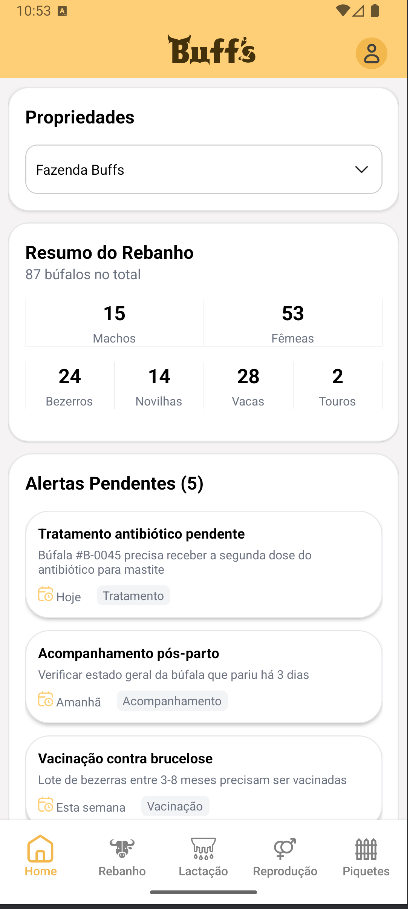
\includegraphics[width=\textwidth]{mobile/home}
    \caption{Tela inícial}
    \label{fig:web_coleta}
\end{subfigure}
\hspace{2cm}
\begin{subfigure}[b]{0.25\textwidth}
    \centering
    \includegraphics[width=\textwidth]{mobile/rebanho}
    \caption{Visualização do rebanho}
    \label{fig:web_piquete}
\end{subfigure}
\SourceOrNote{Autoria Própria (2025)}
\end{figure}


\begin{figure}[!h]
\caption{Exemplos de telas da plataforma web, mostrando indicadores, piquetes e inventário do rebanho}
\centering
\label{fig:web}
\begin{subfigure}[b]{0.437\textwidth}
    \centering
    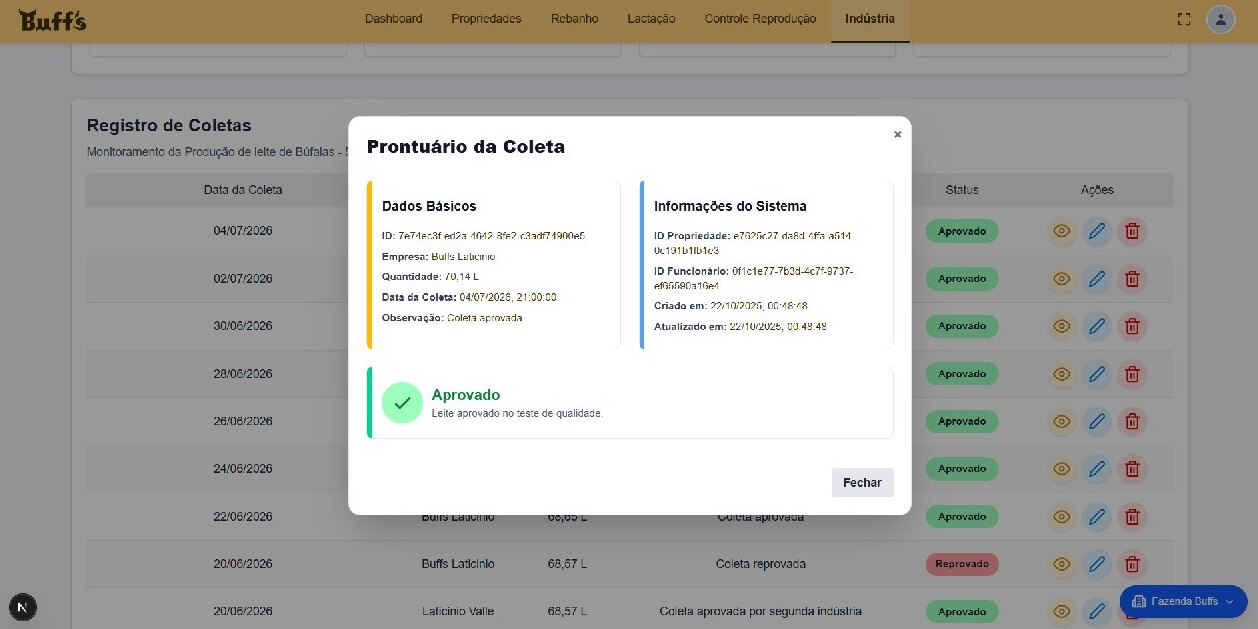
\includegraphics[width=\textwidth]{web/coleta}
    \caption{Feedback de uma coleta}
    \label{fig:web_coleta}
\end{subfigure}
\hfill
\begin{subfigure}[b]{0.437\textwidth}
    \centering
    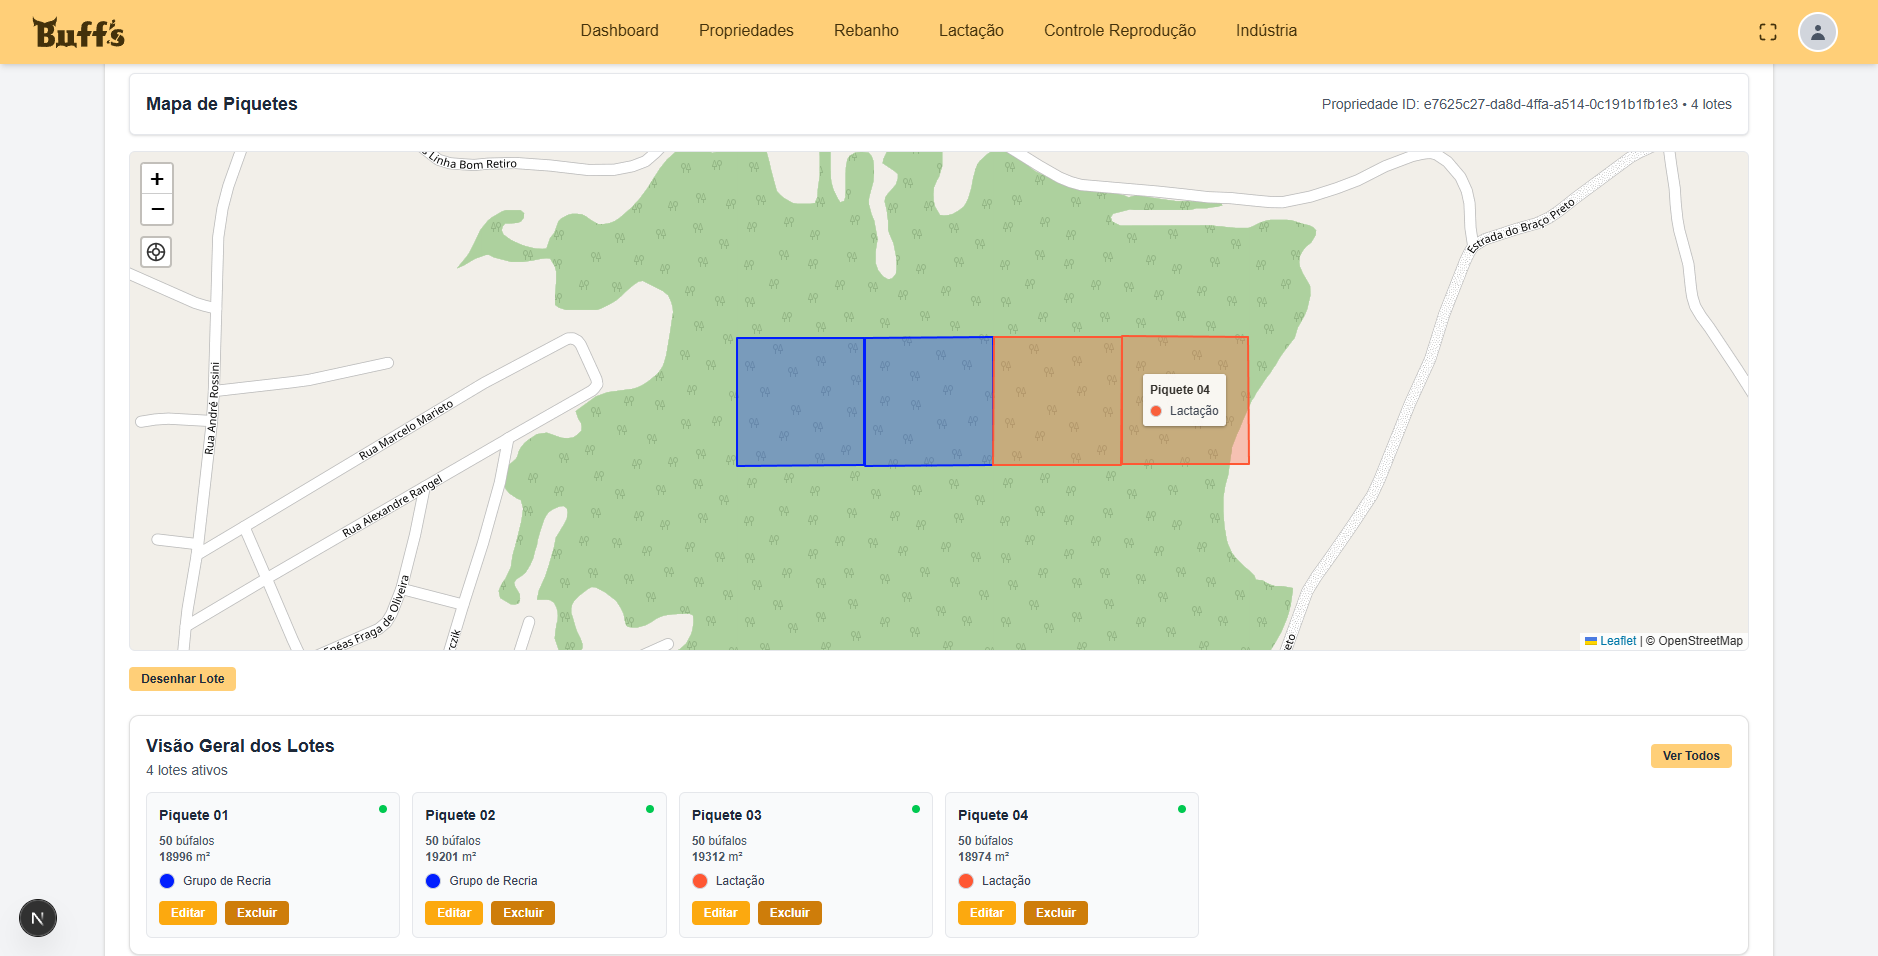
\includegraphics[width=\textwidth]{web/piquete}
    \caption{Visualização de piquetes}
    \label{fig:web_piquete}
\end{subfigure}

\vspace{0.5cm} % Espaço entre linhas

\begin{subfigure}[b]{0.45\textwidth}
    \centering
    \includegraphics[width=\textwidth]{web/rebanho}
    \caption{Visualização do rebanho}
    \label{fig:web_rebanho}
\end{subfigure}

\label{fig:web_exemplos}
\SourceOrNote{Autoria Própria (2025)}
\end{figure}



No \Cref{fcht:fluxograma1} é possivel verificar o fluxo que o Funcionário/Veterinário vão seguir, ao acessa o sistema por meio do aplicativo móvel, por onde realiza a inserção e consulta de informações zootécnicas, sanitárias, reprodutivas e produtivas. Durante o registro de uma nova ordenha, o sistema ativa automaticamente a inteligência artificial(IA) generativa Gemini, que analisa os dados inseridos e identifica descrições compatíveis com mastite. Quando uma ocorrência é constatada, a IA classifica seu nível de gravidade, emitindo alertas que orientam o usuário quanto à urgência de intervenção. Essa abordagem automatizada reduz o risco de omissões, padroniza decisões e agiliza o tratamento clínico, garantindo maior confiabilidade ao processo. As inserções de dados realizadas pelo aplicativo são enviadas à Interface de Programação de Aplicações, do inglês \textit{Application Programming Interface} (API), que as processa e atualiza no banco de dados principal. Esses registros alimentam também a segunda inteligência artificial do projeto, baseada no algoritmo Random Forest Regressor, utilizada para realizar predições da produção leiteira de cada animal.

\begin{flowchart}[!htb]
\centering
\caption{Fluxograma visão do Funcionário/Veterinário}%
\label{fcht:fluxograma1}
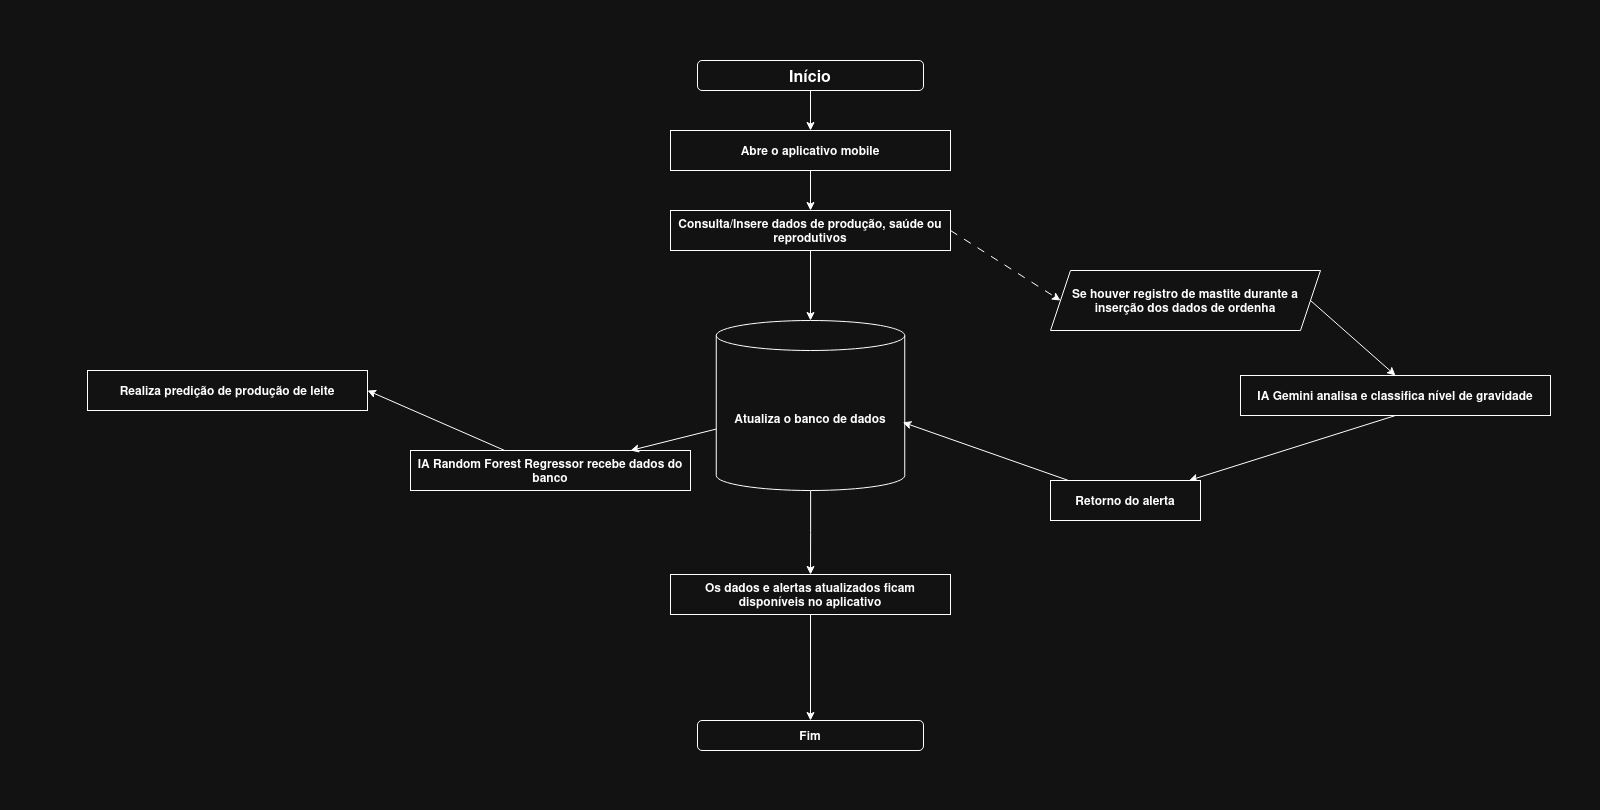
\includegraphics[scale=0.25]{diagrama_funcionario}
\SourceOrNote{Autoria Própria (2025)}
\end{flowchart}

Já no \Cref{fcht:fluxograma2}, o usuário acessa a plataforma web, onde são disponibilizados painéis interativos que apresentam indicadores consolidados de produtividade, sanidade e distribuição do rebanho. Nessa interface, o gestor pode consultar o prontuário individual dos animais, visualizar as predições geradas pela IA de regressão e acompanhar os alertas oriundos da análise de mastite. Caso necessário, é possível inserir ou atualizar informações diretamente pela plataforma web, mantendo a consistência do banco de dados sem a necessidade de acesso ao aplicativo móvel. Essa estrutura integrada permite que o gestor acompanhe em tempo real o desempenho produtivo da propriedade, utilizando dados concretos e análises automatizadas para fundamentar suas decisões de manejo e de investimento.

\begin{flowchart}[!htb]
\centering
\caption{Fluxograma visão do Proprietário/Gestor}%
\label{fcht:fluxograma2}
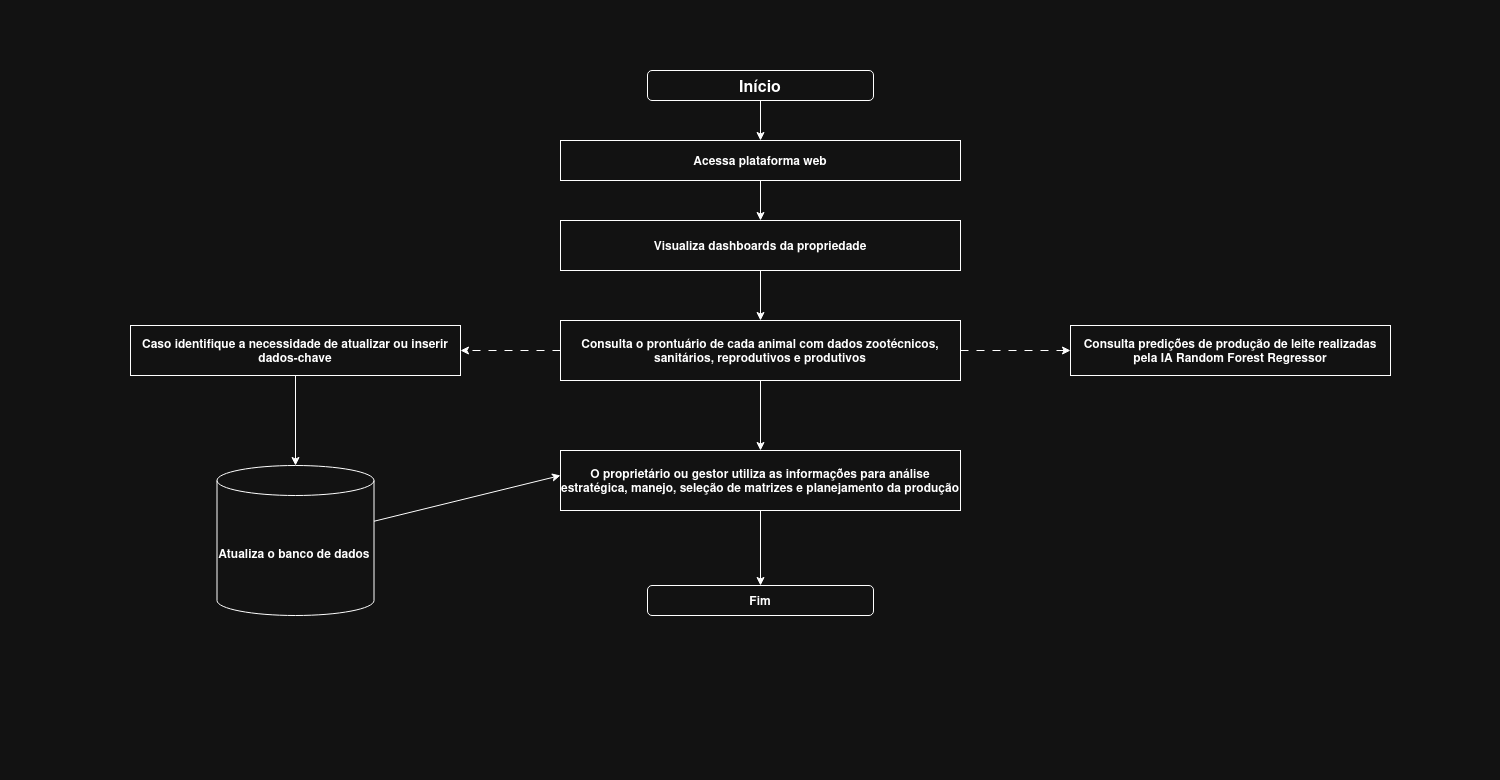
\includegraphics[scale=0.25]{diagrama_propreitario}
\SourceOrNote{Autoria Própria (2025)}
\end{flowchart}

Foi apresentado, anteriormente, toda a fundamentação teórica referente ao fluxo de funcionamento do sistema. Para que esse fluxo ocorra de forma adequada, é necessário o uso de um conjunto de ferramentas e tecnologias que viabilizam a comunicação entre as diferentes camadas da aplicação, conforme ilustrado na \Cref{fcht:arquitetura}. A interação com o usuário inicia-se nas etapas I e II. A Etapa I corresponde à plataforma web, desenvolvida em \textit{React} com o framework \textit{Next.js}. Atualmente, essa plataforma encontra-se hospedada na Vercel, uma solução \textit{serverless} que dispensa a necessidade de um servidor dedicado. A Etapa II refere-se à plataforma mobile, desenvolvida em \textit{React Native}, framework que consiste em um conjunto de ferramentas voltadas à criação de aplicações móveis nativas \cite{Bruna2021}. O aplicativo tem como principal funcionalidade oferecer uma interface simplificada e intuitiva, voltada ao lançamento de dados em campo.

Ambas as plataformas comunicam-se com o Back-end (etapa III) por meio de uma API, desenvolvida em \textit{TypeScript} com o framework \textit{Nest.js}. Como parte do Back-end, foram implementados recursos adicionais com o objetivo de aperfeiçoar a usabilidade e a fluidez do sistema, destacando-se a integração com dois modelos de Inteligência Artificial(IA). A primeira delas é a API \textit{Gemini} (etapa IV), um modelo generativo multimodal desenvolvido pelo Google. No contexto deste projeto, a \textit{Gemini} é utilizada no sistema de alertas, por meio do modelo \textit{gemini-1.5-flash}. Essa implementação analisa um \textit{prompt} elaborado especificamente para o domínio do sistema e define a prioridade de cada alerta como alta, média ou baixa, simplificando de maneira significativa a lógica de priorização e resposta.

A segunda IA (etapa V) foi desenvolvida pelo próprio grupo e baseia-se no algoritmo \textit{Random Forest Regressor}, um método de aprendizado supervisionado que combina múltiplas árvores de decisão para realizar previsões numéricas. O modelo é treinado com diversas amostras aleatórias dos dados e, para cada árvore, um subconjunto de atributos, conhecidos como \textit{features}, é selecionado de forma aleatória, promovendo diversidade entre os estimadores. A predição final é obtida a partir da média dos resultados de todas as árvores, aumentando a precisão e reduzindo o risco de sobreajuste, conhecido como \textit{overfitting}, em comparação com o uso de uma única árvore de decisão. No contexto deste trabalho, o modelo tem como objetivo prever individualmente a produção de leite de cada fêmea, utilizando seu histórico produtivo, reprodutivo, sanitário, zootécnico e genético. Essas informações são consolidadas em um conjunto de \textit{features} estruturadas e, a partir delas, o sistema gera uma predição que classifica o potencial produtivo em categorias, sendo elas alto, bom, médio ou baixo. O resultado é ainda comparado com a média da propriedade e fornece informações adicionais, como o volume previsto em litros, o percentual em relação à média e a data da predição.

Para disponibilizar todo o Back-end de forma operacional e acessível, o mesmo foi hospedado na nuvem utilizando o serviço \textit{Amazon EC2}, \textit{Elastic Compute Cloud}, da \textit{Amazon Web Services} (AWS). Essa escolha permite escalar a infraestrutura dinamicamente, otimizando custos e garantindo melhor desempenho do sistema. A API é responsável por gerenciar toda a lógica de negócios, incluindo a criação, consulta, atualização e exclusão de registros no banco de dados, além de processar requisições provenientes das plataformas web e mobile. O controle de \textit{deploy} automático (etapa VI) é realizado por meio do \textit{GitHub Actions}, que integra diretamente com a instância EC2, automatizando atualizações e correções e assegurando que a aplicação permaneça sempre disponível e atualizada para os usuários.

Para o armazenamento das informações, o banco de dados do sistema (etapa VII) foi desenvolvido em \textit{PostgreSQL}, escolhido pela sua robustez e pela consistência oferecida pelo modelo relacional na organização e integridade dos dados. Essa estrutura permite armazenar grandes volumes de informações de forma estruturada, garantindo que registros relacionados, como dados de produção, lactação e histórico sanitário dos animais, sejam mantidos de forma segura e coerente. Atualmente, o banco de dados encontra-se hospedado na nuvem por meio da plataforma \textit{Supabase}, que oferece compatibilidade nativa com o PostgreSQL, além de recursos adicionais de autenticação e armazenamento.

\begin{flowchart}[!htb]
\centering
\caption{Arquitetura do fluxo das redes}%
\label{fcht:arquitetura}
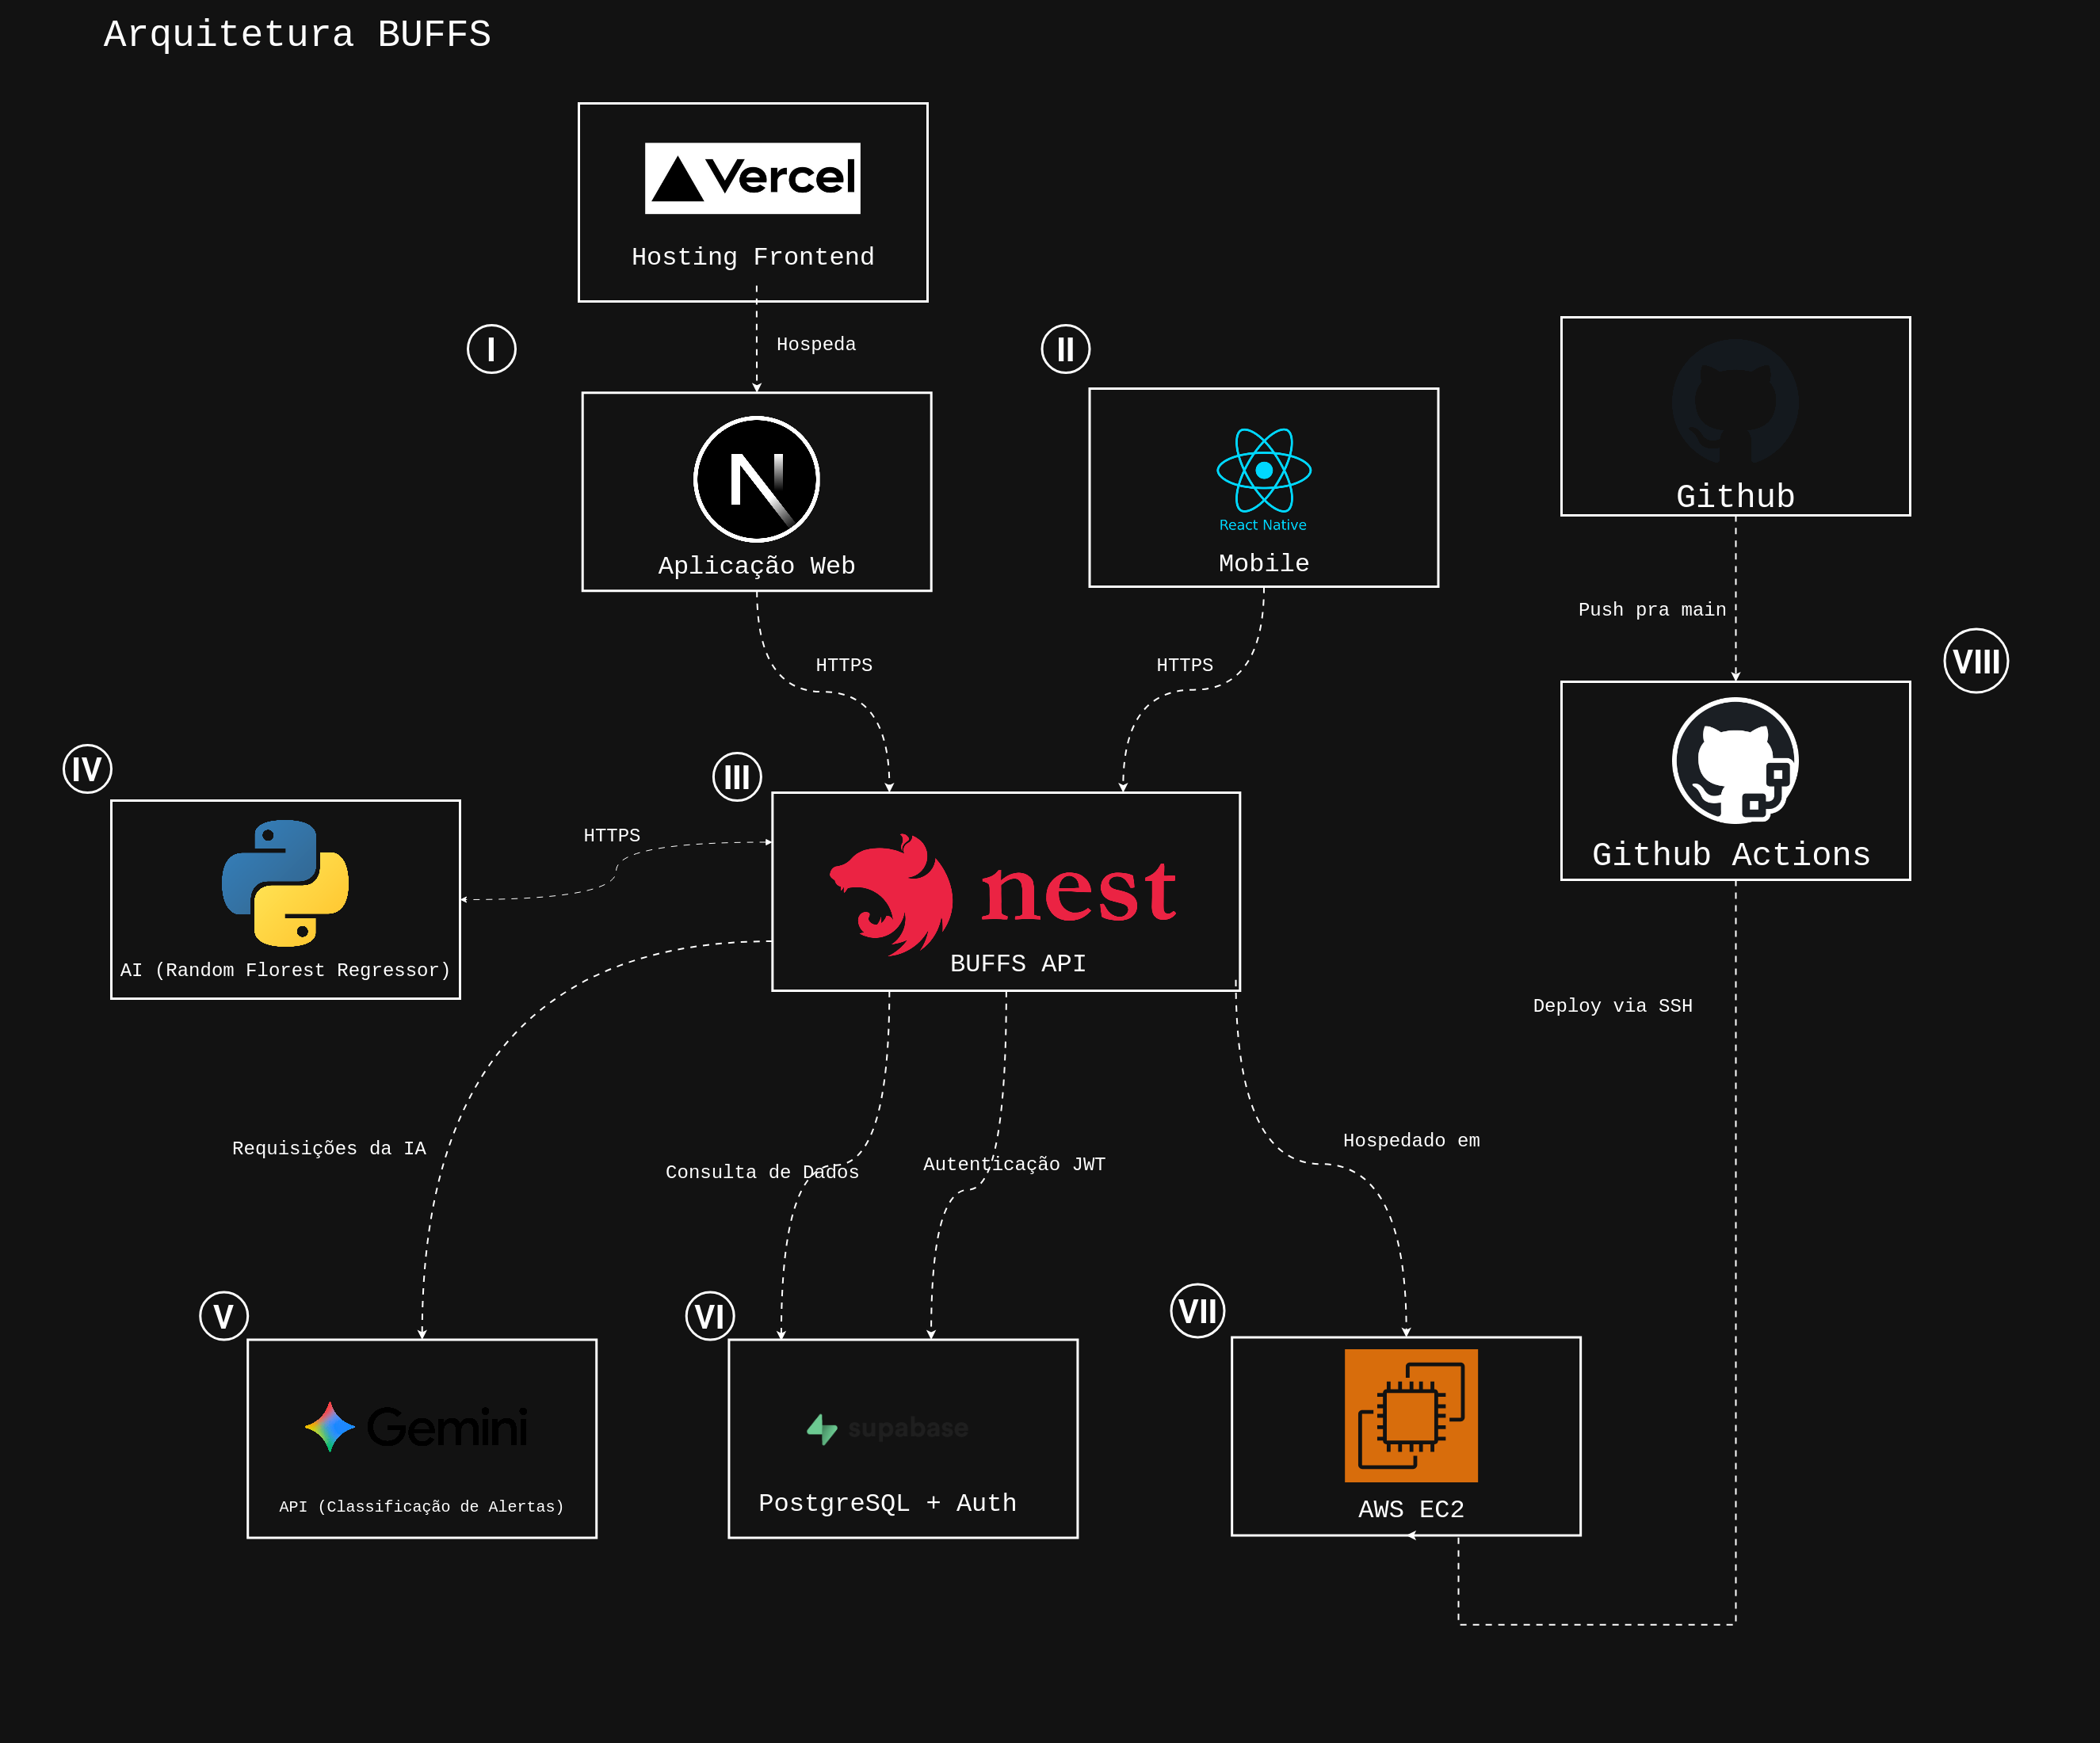
\includegraphics[scale=0.15]{buffs-arch-model}
\SourceOrNote{Autoria Própria (2025)}
\end{flowchart}

Após a análise do fluxo apresentado, nota-se que grande parte do sistema encontra-se hospedada na nuvem, seja por meio de serviços \textit{serverless}, bancos de dados em ambiente \textit{cloud} ou máquinas virtuais dedicadas. Essas escolhas, no momento atual, mostraram-se adequadas sob a ótica do grupo, uma vez que permitem distribuir as \textit{stacks} entre diferentes serviços, evitando a sobrecarga de um único sistema. Além disso, essa configuração possibilita a realização de testes de forma gratuita, sem a necessidade de investimentos iniciais em infraestrutura. Outro fator determinante nas decisões de arquitetura foi o alinhamento com os conteúdos abordados em sala de aula, privilegiando tecnologias e metodologias com as quais o grupo possui maior afinidade e embasamento técnico. Essa estratégia busca não apenas consolidar o aprendizado adquirido ao longo do curso, mas também garantir que o desenvolvimento ocorra de maneira segura e fundamentada em conhecimentos previamente assimilados.
